\documentclass[a4paper,12pt]{report}

\usepackage[utf8]{inputenc} % damit auch äöüß gehen
\usepackage[T1]{fontenc}	% so kann man bessere wörtliche rede machen
\usepackage[ngerman]{babel} % deutsche Silbentrennung
\usepackage{SIunits} % SI Einheiten
\usepackage{csvsimple} % for tables
\usepackage{graphicx}
\usepackage{amsmath}
\usepackage{subcaption} % Figures mit mehr als einem Bild
\usepackage{enumitem} % um aufzählungen zu machen
\usepackage{todonotes}
\usepackage[left=3cm, right=3cm]{geometry}
\usepackage{tocloft}

\usepackage[
	colorlinks,
	pdfpagelabels,
	bookmarksopen = true,
	bookmarksnumbered = true,
	linkcolor = black,
	urlcolor = blue,
	plainpages = false,
	hypertexnames = false,
	citecolor = black
]{hyperref} % verlinkt referenzen für die digitale verwendung

\newcommand{\au}{\glqq}
\newcommand{\ao}{\grqq\ } % anführungsstriche

%%% FOR FANCY GRAPHS %%%
\usepackage{tikz}
\usetikzlibrary{arrows,shadows,positioning, arrows.meta, automata}
\tikzset{
	frame/.style={
		rectangle, draw, 
		text width=6em, text centered,
		minimum height=4em,drop shadow,fill=lime!40,
		rounded corners,
	},
	line/.style={
		draw, -latex',rounded corners=2mm,
	}
}
\usepackage{pgfplots}
\usetikzlibrary{datavisualization}
\usetikzlibrary{datavisualization.formats.functions}

\usepackage{titlepic} % mit Bild auf der Titelseite

\begin{document}

%%%%%%%%%%%%%%%%%%%%% HEADER %%%%%%%%%%%%%%%%%%%%%

	\title{Workshop VHDL B143a\\Fachhochschule Wedel}
	\author{Guillaume Fournier-Mayer (Tinf 101922) \\
		Jan Ottmüller (Tinf101737)}
	\date{\today}
	\maketitle

	\setlength{\cftbeforechapskip}{0.1em}
	\tableofcontents


%%%%%%%%%%%%%%%%%%%%%%%%%%%%%%%%%%%%%%%%%%%%%%%%%%

\chapter{Einleitung}
	Diese Dokumentation dokumentiert und beschreibt den Workshop VHDL (B143a).\\
	Die Aufgabe dieses Semesters mit dem Namen \au Crypto Notepad\ao erfordert das Auslesen einer PS2 Tastatur, die Ver- und Entschlüsselung sowie Speicherung der Tastaturausgaben und das Ausgeben des Speichers auf einem Zwei-Zeilen-Textdisplay.\\
	Die Beschreibung soll auf dem Altera DE2 board mit Cyclone 2 FPGA laufen.  

\chapter{Aufgabenanalyse}
	Für die Implementierung haben wir uns folgende Ziele gesetzt:
	\begin{enumerate}
		\item Gute Modularisierung zur Wiederverwendbarkeit der einzelnen Module
		\item Klare Namensgebung der Signale und Prozesse
		\item Die Top-Level-Entity soll im RTL-Viewer übersichtlich und strukturiert sein. 
	\end{enumerate}
	Ausgehend von der Top-Level-Entity (TLE) sollen die einzelnen Komponenten eingebunden und verbunden werden.\\
	Die Top-Level-Entity CryptoNotepad enthält somit Schnittstellen zum Board und führt die einzelnen Module zusammen.\\
	Hier die Grobe Strukturierung der Entities auf TLE:\\
	\begin{center}
		\begin{tikzpicture}[font=\small\sffamily\bfseries,very thick,node distance = 4cm, scale=0.8, every node/.style={scale=0.8}]
		
		\node [frame] (key) {Keyboard};
		\node [frame, right of=key] (cry) {Crypto};
		\node [frame, below=-1cm, below of=cry] (ram) {RamAccess};
		\node [frame, right of=cry] (dis) {Display};
		\node [left of=key, above=0.5cm] (in) {PS2};
		\node [above of=cry, above=-1cm] (incry) {Schlüssel};
		\node [right of=dis, above=0.5cm] (out) {Display Bus};
		
		\path [line, <->] (in) |-  (key);	
		\path [line, ->] (key.90) |- node[above,pos=.75, align=center] {PS2 Code} +(3.5,1) to (cry.120);
		\path [line, <->] (ram) to (cry);
		\path [line, ->] (cry.60) |- node[above,pos=.75, align=center] {entschlüsselte \\ Daten} +(3.5,1) to (dis.90);
		\path [line, ->, rotate=90] (dis.0) |- (out.270);
		
		\path [line, ->] (key) |- node[above,pos=.75, align=center] {erhöhe \\ writeaddress} (ram);
		\path [line, ->] (incry) to (cry);
		\path [line, ->] (dis) |- node[above,pos=.75, align=center] {erhöhe \\ readaddress} (ram);
		\end{tikzpicture}
		\captionof{figure}{Vereinfachtes Blockschaltbild TLE}
	\end{center}
	Die Entity RamAccess dient als Schnittstelle zum, mit dem MagicWizzard automatisch generiertem, Ram.\\
	Die Ver- und Entschlüsselung der Zeichen soll in einer separaten Entity stattfinden um das Problem besser zu modularisieren und die Keyboard Entity möglichst wiederverwendbar zu machen. Diese gibt über ihren Ausgang die empfangenen Scancodes aus. Ein andere Möglichkeit wäre, die PS2 zu ASCII Konvertierung bereits im Keyboard Modul durchzuführen. Jedoch ist diese Umwandlung auch eine Art Verschlüsselung und findet deshalb in der Crypto Entity Platz.\\
	An vielen Orten sollen Zustandsautomaten mit zwei- oder drei-Prozess-Beschreibung verwendet werden. Spezielle Zustandstypen sollen die Übersichtlichkeit fördern.\\
	Die Keyboard Entity wird in Transmitter und Receiver aufgeteilt.\\
	Das Display ist deutlich langsamer als der FPGA. Um dies zu berücksichtigen, können zwei Strategien verfolgt werden. Entweder kann das Busy Signal vom Display ausgelesen werden. Wenn das Display bereit ist, wird dieses ausgeschaltet und es können neue Daten gesendet werden. Ein anderer Ansatz macht sich zu Nutzen, dass wenn man lange genug wartet, das Display immer bereit ist. So wird das Display nach 2,5\,ms (400\,Hz) immer fertig mit der Verarbeitung des letzten Befehls sein. \\
	In der Initialisierungsphase kann das Busy Signal jedoch nicht ausgelesen werden, weshalb der zweite Ansatz gewählt wird.\\
	
	
	\section{Zusatzaufgabe}
		Um kleinere Fehler in der Implementierung auszugleichen, soll eine Zusatzfunktion implementiert werden, welche die Aufgabe erweitert.\\
		Eine Erweiterung, welche implementiert wird, ist das Setzen der Status-LEDs. Hierfür muss der PS2-Transmitter funktionieren, da Kommandos an die Tastatur verschickt werden müssen. Diese Funktion soll im Keyboard Modul Platz finden.   
	
\chapter{Benutzerhandbuch}
	\section{Reset}
		Die Schaltung kann über den Schalter SW17 zurückgesetzt werden. Hierbei werden alle Zustände der Schaltung zurückgesetzt. Als letztes muss der PS2 Stecker neu eingesteckt werden, damit auch die Status LEDs an der Tastatur zurückgesetzt werden.\\
		Ein Zurücksetzen des Speichers, und somit des Displayinhaltes geschieht nicht. Jedoch wird der Cursor wieder auf das Erste Feld im Display gesetzt, wenn der PS2 Stecker neu eingesteckt wird.
		
	\section{Anwendung}
		Nachdem das Programm auf das Altera DE2 Board geladen wurde, wird die Tastatur angeschlossen. 
		Danach können Zeichen über die angeschlossene Tastatur eingegeben werden. Sie werden auf das Display geschrieben. Zulässig sind die Tasten a-z sowie 0-9 und 'LEERZEICHEN'. Bei nicht bekannten Zeichen wird ein \au ?\ao ausgegeben.	 
		Beim Drücken auf die Tasten CAPS-LOCK, SCROLL-LOCK, und NUM-LOCK gehen die entsprechenden Status LEDs auf der Tastatur an und bei erneutem Drücken wieder aus. Einen Einfluss auf die geschriebenen Zeichen gibt es nicht.\\
		Über die Schalter SW0 bis SW7 kann der zu verwendende Schlüssel eingegeben werden, mit dem die Daten vor dem Speichern verschlüsselt, und beim Lesen entschlüsselt werden. Die Verschlüsselung ist eine einfache XOR Verknüpfung. Der Schlüssel kann nach belieben geändert werden. Die Zeichen auf dem Display werden entsprechend des eingestellten Schlüssels entschlüsselt und auf dem Display angezeigt.

\chapter{Implementierung}
	In diesem Kapitel werden die Entities Bottom-Up beschrieben.

	\section{DoubleEdgeDetector}
		Diese Entity erledigt die Einsynchronisierung der PS2 Takt und Datenleitung. Hierfür werden hintereinander geschaltete Flip Flops verwendet, sodass Metastabilität im System vermieden wird, wenn das Signal zu einem ungünstigen Zeitpunkt empfangen wird. Als weitere Ausgänge verfügt der Edge Detector über zwei Signalausgänge. Das Signal fedge\_o wird bei Fallender Flanke des Eingangs für einen Takt auf 1 gesetzt. Das Signal redge\_o bei steigender Flanke.
		
	\section{Transmitter}
		\begin{figure}[h]
		\centering
		\begin{tikzpicture}[->,>=stealth',shorten >=1pt,auto,node distance=2.8cm,
		semithick]
		\tikzstyle{every state}=[fill=lime!40,thick,draw=none,text=black]
		
		\node[initial,state,label={above:$WaitToSend$}] (A) {$Q_0$};
		\node[state,label={above:$PullClkLow$}]         (B) [right of=A] {$Q_1$};
		\node[state,label={above:$PullDatLow$}]         (C) [right of=B] {$Q_2$};
		\node[state,label={below:$SendFirstBit$}]       (D) [below of=C] {$Q_3$};
		\node[state,label={below:$Send$}]               (E) [left of=D] {$Q_4$};
		\node[state,label={below:$CheckTimeout$}]       (F) [left of=E] {$Q_5$};
		\node[state,label={below:$CleanUp$}]            (G) [left of=F]  {$Q_6$};
		
		\path (A) edge (B);
		\path (B) edge (C);
		\path (C) edge (D);
		\path (D) edge (E);
		\path (E) edge (F);
		\path (F) edge (G);
		\path (D) edge (A);
		\path (E) edge (A);
		\path (F) edge (A);
		\path (G) edge (A);
		\end{tikzpicture}
		\caption{Zustandsautomat Transmitter}
	\end{figure}
	Beim Senden werden die PS2-Clockimpulse von der Tastatur erzeugt. Zum Senden muss der Host die Leitungen in den Request-To-Send Zustand bringen, indem die Clock Leitung für 100$\mu$s auf Low zieht und danach die Datenleitung auch auf Low zieht und beide wieder freigibt.\\
	Die Tastatur generiert nun Clockimpulse bei denen die Daten vom Host gesendet werden. Das ändern der Daten geschieht bei Low Pegel. Das Auslesen von der Tastatur geschieht bei High Pegel. Hierbei können zwei Timeouts auftreten. Entweder Die Tastatur fängt erst später als 15ms an, den Takt zu generieren, oder die Übertragung des Datenpaketes dauert mehr als 2ms. Diese Zeitmessung wird bei der Implementierung in der Entity berücksichtigt.\\
	Der Kern dieser Entity ist ein Zustandsautomat in Zwei-Prozess-Beschreibung.\\
	
	
	\section{Receiver}
		Im Gegensatz zum Senden werden beim Empfangen die Daten bei Fallender PS2 Clock Flanke vom Host gelesen. Bei diesem Ereignis wird der anliegende Pegel des PS2 Datensignals in das Schieberegister \textit{regs} geschrieben, welches danach weitergeschoben wird. Sind alle 11 Bits eines PS2 Paketes empfangen, so wird geprüft, ob die logische Verknüpfung mit dem Ergebnissignal \textit{error} einen Fehler signalisiert. Entsprechend der Auswertung werden die Daten dann an den Datenausgang der Entity geschrieben und das Empfangen eines neuen Paketes signalisiert.
	\section{Transceiver}
		Der Transceiver implementiert das Senden und Empfangen von Daten über die PS2 Schnittstelle. Hierfür werden die Komponenten Transmitter und Receiver eingebunden. Die PS2 Signale werden mit Hilfe von DoubleEdgeDetectoren ein-synchronisiert. Da die ein-synchronisierten Signale, sowie die Flankendetektoren, wie in Abb. \ref{fig:trans} mit gestrichelten Linien zu sehen, sowohl im Receiver als auch im Transmitter benötigt werden, sind Die Flankendetektoren auf dieser Ebene implementiert. 
		\begin{center}
			\begin{tikzpicture}[font=\small\sffamily\bfseries,very thick,node distance = 4cm, scale=0.8, every node/.style={scale=0.8}]
				
				\node [frame] (dedclk) {Edge Detector \\ PS2-Clk};
				\node [frame, below of=dedclk] (deddat) {Edge Detector \\ PS2-Data};
				\node [frame, below=0.5cm, right of=dedclk] (tra) {Transmitter};
				\node [frame, above =0.5cm, right of=deddat] (rec) {Receiver};
				\node [left of=deddat, below=0.5cm] (ind) {PS2-Data};
				\node [left of=dedclk, above=0.5cm] (inc) {PS2-Clock};
				\node [below of=inc, below=-1cm] (in) {In-Data};
				\node [right of=in, right=6cm] (out) {Out-Data};
				
				
				\path [line, ->] (ind) |-  (deddat);
				\path [line, ->] (inc) |-  (dedclk);
				\path [line, ->] (in)  |-  (rec.160);
				\path [line, ->] (in)  |-  (tra.200);	
				\path [draw, ->,dashed] (dedclk.355) |- (tra.160);
				\path [line, ->, dashed] (dedclk.355)+(0.6,0)  |- (rec.200);
				\path [draw, ->, dashed] (deddat.5) |- (rec.200);
				\path [line, ->,dashed] (deddat.5) +(0.4,0) |- (tra.200);
				
				\path [line, ->, rotate=90] (tra.0) |-  (out);
				\path [line, ->, rotate=90] (rec.0) |-  (out);
				\end{tikzpicture}
				\captionof{figure}{Blockschaltbild Transceiver}
				\label{fig:trans}
			\end{center}		
	\section{Keyboard}
		
	\section{Crypto}
	Die Entity Crypto dient zum Ver- und Entschlüsslen der Daten. Sie Enthält keine internen Signale oder Speicherzustände und bedarf deswegen keinem Takt und Reset Signal. Die Umsetzung der Make codes in ASCII Zeichen findet ebenfalls hier statt. Dies mag auf den ersten Blick keine Verschlüsselung sein, doch genauer Betrachtung ist diese Umwandlung auch nur eine Art der Verschlüsselung. Anschließend wird das ASCII Zeichen mit dem übergebenen Schlüssel XOR verknüpft und zurückgegeben.\\
	Bei der Entschlüsselung findet wieder eine XOR Verknüpfung mit dem anliegenden Schlüssel statt.
	
	\section{RamAccess}
		Die Entity RamAccess dient als Schnittstelle zum Ram. Es werden hilfreiche Schnittstellen zur Traversierung des Speichers bereitgestellt.\\
		Da sowohl das Schreiben, als auch das Lesen des Speichers in einer definierten Reihenfolge stattfindet, kümmert sich diese Entity um diese Aufgabe. Bei Steigender Flanke an den Signalen \\ \textit{ramaccess\_increase\_read\_address} und \textit{ramaccess\_increase\_write\_address} werden die entsprechenden Adressen erhöht. Zur Detektierung der Flanken wird der bereits implementierte DoubleEdgeDetector benutzt, da die Signale für mehrere Taktzyklen an sind, aber die Adresse nur einmal inkrementiert werden soll. Die leichte Verzögerung des Signals durch den Kantenerkennung ist nicht störend. Beim Inkrementieren der Schreibadresse wird mit Einschalten des Signals ram\_write\_enable der Inhalt des Dateneingangs in den Speicher geschrieben.
		\begin{center}
			\includegraphics[width=1\textwidth]{assets/RamAccess}
			\captionof{figure}{RamAccess Modul RTL Ansicht}
		\end{center}
	
	\section{Ram}
		Das Ram Modul ist ein, mit dem Magic Wizzard automatisch generierter, Speicherbaustein. Dieser besitzt mit 8Bit x 32Bit genauso viele Bytes wie das Display Zeichen hat. So kann man eine direkte Abbildung des Speichers auf dem Display realisieren. Leider verfügt das Ram Modul nicht über einen Asynchronen Reset, welcher den ganzen Speicher leert. Dies wäre praktisch, um den Display Inhalt bei einem Reset zu leeren.
	
	\section{Display}
	
		\begin{figure}[h]
		\centering
		\begin{tikzpicture}[->,>=stealth',shorten >=1pt,auto,node distance=2.8cm,
		thick]
		\tikzstyle{every state}=[fill=lime!40,thick,text=black]
		
		\node[initial,state] (A)              {$init$};
		\node[state]         (B) [right of=A] {$clear$};
		\node[state]         (C) [right of=B] {$off$};
		\node[state]         (D) [right of=C] {$mode$};
		\node[state]         (E) [right of=D] {$on$};
		\node[state]         (F) [below of=E] {$switchC$};
		\node[state]         (G) [left of=F]  {$wait$};
		\node[state]         (H) [left of=G]  {$print$};
		
		\path (A) edge (B);
		\path (B) edge (C);
		\path (C) edge (D);
		\path (D) edge (E);
		\path (E) edge (F);
		\path (F) edge (G);
		\path (G) edge [bend right] (H);
		\path (H) edge [bend right] (G);
		\path (F) edge [bend right] (H);
		\path (H) edge [bend right] (F);
		\end{tikzpicture}
		\caption{Vereinfachter Zustandsautomat ohne Wartezustände}
		\end{figure}
	
		Der Kern der Display Entity ist ein Zustandsautomat der, wie in der Aufgabenanalyse beschrieben, mit einem Takt von 400 Hz getaktet ist.
		
		\subsection{Prozesse}
			Der Zustandsautomat wird mit einer drei-Prozess-Beschreibung implementiert. So entstehen die drei Prozesse \textit{store}, \textit{transition} und \textit{output}. Der vierte Prozess \textit{displayClock} dient der Generierung des Display Taktes. 
		\subsection{Displaytakt}
			Dieser Prozess generiert langsame Impulse mit 400 Hz, indem die Taktzyklen von lcd\_clk\_i gezählt werden. \\Bei 62500 gezählten Taktflanken wird das Signal clk\_displayEnable für einen Takt auf 1 gesetzt, was bei 50 MHz Basistakt zu 400 Hz führt.
		\subsection{Initialisierung}
			In der Initialisierungsphase wird zunächst für 10ms das Function Set Signal an den parallelen Bus angelegt. das Signal lcd\_rs steht auf 0, da die Daten auf das Controll Register und nicht auf das Datenregister geschrieben werden sollen. Im Function Set wird der Display Controller auf einen 8-Bit Bus mit einem Zweizeilen Display initialisiert.\\
			Danach wird das Display ausgeschaltet und der Inhalt gelöscht.
			Jetzt folgen die entsprechenden Befehle, um den Cursor automatisch weiter zu setzen und den Cursor anzuzeigen.
			Abschließend wird das Display wieder eingeschaltet.
		\subsection{Zeichen schreiben}
			Nach der Initialisierungsphase können Zeichen als ASCII Code an das Display gesendet werden. Hier wechseln sich nun immer die Zustände printChars und waitState ab, es sei denn, der Cursor befindet sich am Ende des Displays und muss die Displayzeile wechseln.
			im Zustand PrintChars wird über lcd\_rs das Datenregister zum schreiben ausgewählt und die Daten vom Datenbus lcd\_ram\_data\_i werden in den Speicher des Displays geschrieben. Im waitState wird dann über die ausgehende Schnittstelle das Ram\_Access Modul dazu angewiesen, die Leseadresse des Speichers zu erhöhen. 
		\pagebreak
	\section{CryptoNotepad}
		Diese Entity ist die Top-Level-Entity.
		Von hier aus werden die einzelnen Module verknüpft und die Pins an den FPGA verschaltet.
		\begin{center}
			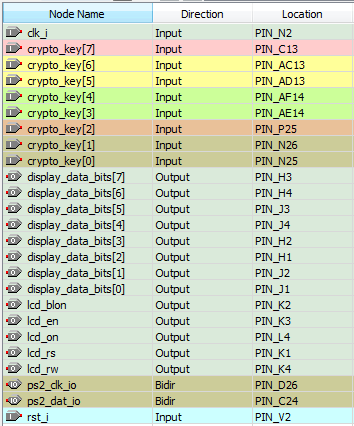
\includegraphics[width=0.6\textwidth]{assets/io}
			\captionof{figure}{Pin Zuweisung im Pin Planner}
		\end{center}
		

\chapter{Test}
	Für das Testen der Funktionalität der einzelnen Entities werden Testbenches geschrieben, welche in Modelsim simuliert werden.
	Zunächst werden die grundlegenden Entities getestet. Sobald diese als funktionstüchtig festgestellt sind, werden Testbenches für die Entities geschrieben, welche die grundlegenden Funktionen zusammenführen. So kann an dieser Stelle die Zusammenarbeit der einzelnen Entities getestet werden.
	
	\section{DoubleEdgeDetector\_tb}
		Aufgrund der recht einfachen Funktionalität der Entity ist auch die Testbench recht klein. An den Eingang wird ein sich änderndes Signal angelegt. Mit Asserts werden dann die Zustände der eingetakteten Signale überprüft.
		\begin{center}
			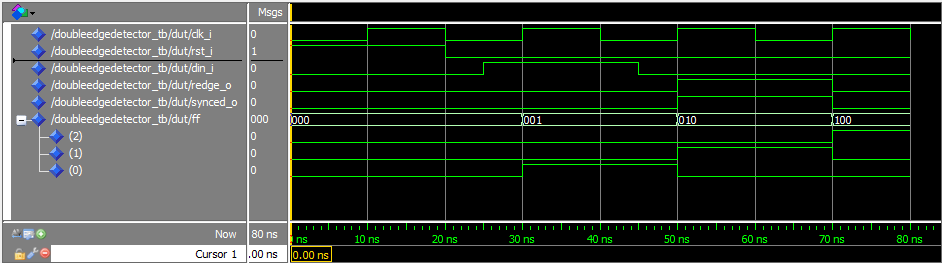
\includegraphics[width=1\textwidth]{assets/DoubleEdgeDetector_tb}
			\captionof{figure}{Signalverlauf DoubleEdgeDetector Testbench}
		\end{center}
	
	\section{Transceiver\_tb\_receiver}
		Zum Testen des PS2 Empfängers werden zwei Pakete Simuliert. Das erste ist ein aalides Paket. Mit Asserts wird geprüft, ob die entsprechenden Signale richtig gesetzt sind. 
		Auf das erste Paket folgend wird ein Paket mit fehlerhafter Parität gesendet. Daraufhin wird geprüft, ob das Fehlersignal an geht und nicht fälschlicher Weise signalisiert wird, dass neue Daten empfangen wurden. 
		Der System und PS2 Takt werden in separaten Prozessen erzeugt.
		\begin{center}
			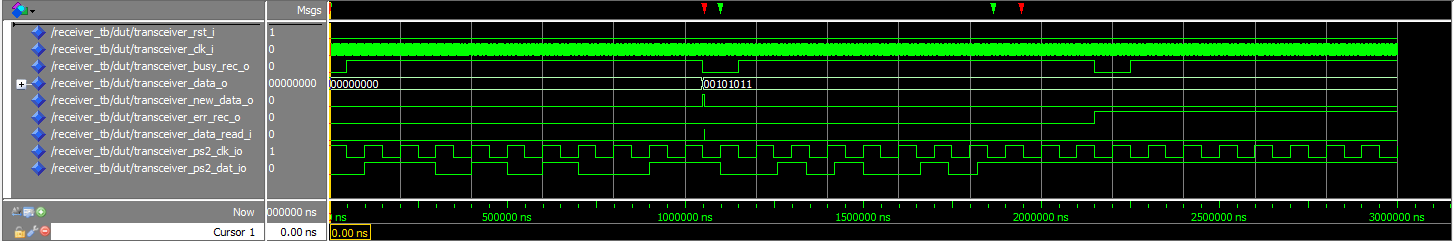
\includegraphics[width=1\textwidth]{assets/receiver_tb}
			\captionof{figure}{Signalverlauf DoubleEdgeDetector Testbench}
		\end{center}
	
		\pagebreak
	\section{Transceiver\_tb\_transmitter}
		Zum Testen des Transmitters wird das Versenden von zwei Paketen simuliert. Da beim Senden der Takt von der Tastatur erzeugt wird, muss der Takt in der Testbench simuliert werden.\\
		Während des Sendevorgangs werden die PS2-Daten mitgeschnitten und am Ende des Tests mit den gesendeten Daten verglichen.\\
		Danach wird ein Fehlerfall simuliert, indem der PS2 Takt als deutlich zu langsam simuliert wird. Hier wird nach 2ms ein Timeout ausgelöst.
		
		Nachdem das Simulieren in der Testbench funktionierte, wurde der Transceiver auf der Hardware getestet. Leider schlug dies fehl und die Tastatur begann zu Blinken, da ein Fehler bei der Übertragung auftrat. Deswegen wurden die PS2 Daten und Clock Leitungen auf zwei LED Ausgänge des Boards Herausgeführt, um sie mit dem Oszilloskop abzugreifen. Die Signalverläufe wurden dann mit der Testbench abgeglichen und entsprechend angepasst. Der Fehler war, dass die Tastatur direkt nach dem Versenden eines Paketes noch nicht bereit zum Empfangen eines neuen Paketes war. Als Lösung wird nun vor dem Versenden der Daten 400\,$\mu$s gewartet
		\begin{center}
			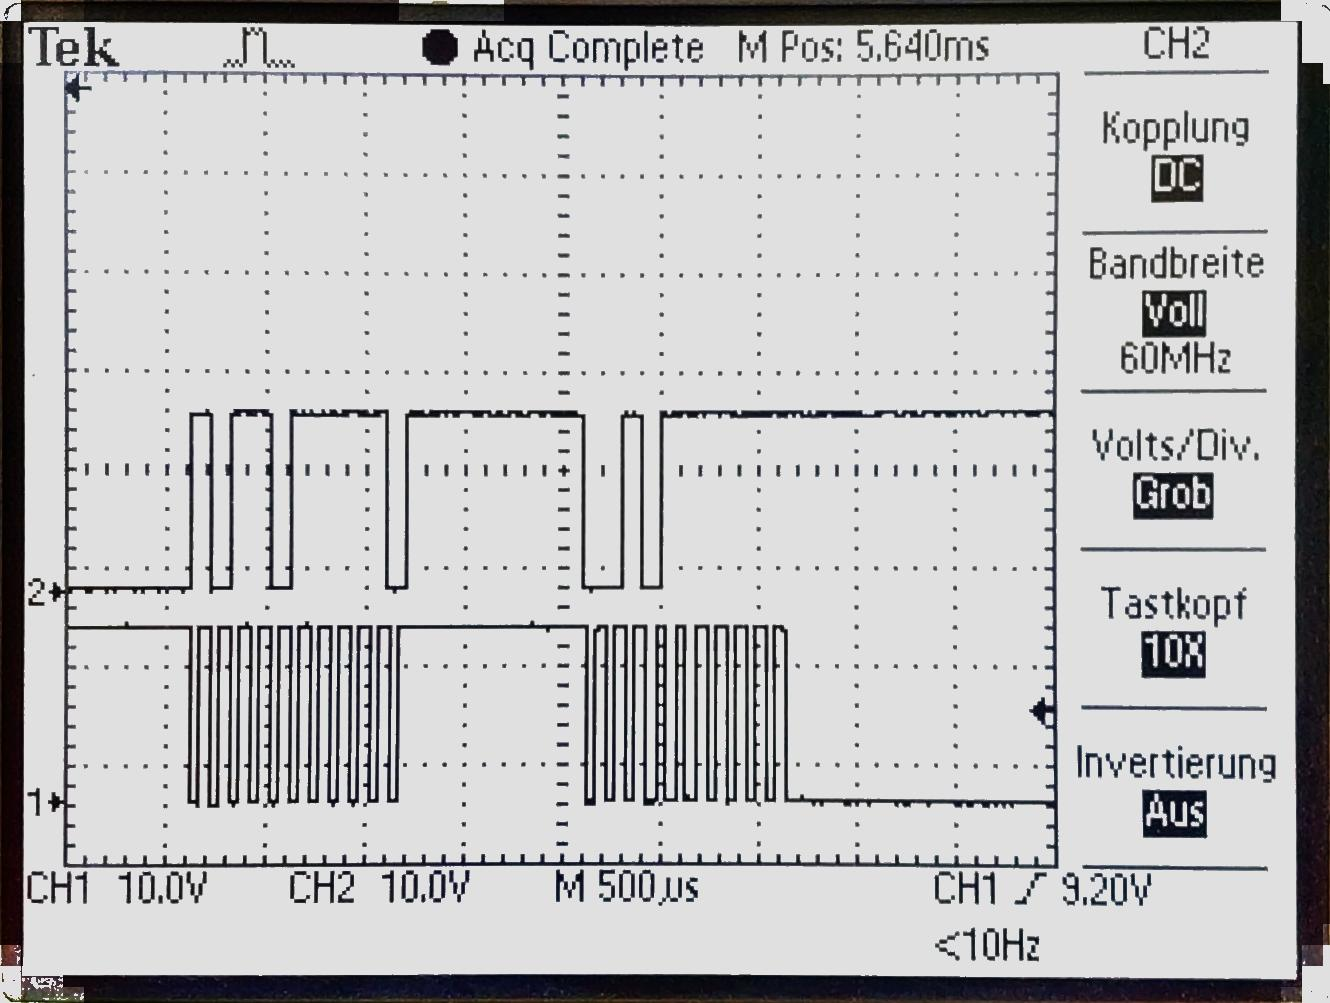
\includegraphics[width=0.7\textwidth]{assets/osz-numLock}
			\captionof{figure}{NumLock paket mit gesendetem \ao 0xED\ao paket zum Einstellen der LEDs}
		\end{center}
		\begin{center}
			\includegraphics[width=1\textwidth]{assets/transmitter_tb}
			\captionof{figure}{Signalverlauf Transmitter Testbench}
		\end{center}
	
	\section{Keyboard\_tb}
		Da die Funktionalität das Transceivers schon getestet wurde, wird in der Keyboard Testbench das Einschalten der NumLock Taste simuliert.\\
		Zunächst wird der Tastendruck der NumLock Taste simuliert. Danach wird das Taktsignal zum Senden des 0xED Paketes erzeugt, da dies sonst die Tastatur übernimmt. Nachdem das simulierte ACK  Paket empfangen wurde wird wieder der Takt für das Paket gesendet, mit dem Die LED an der Tastatur eingeschaltet werden.
		\begin{center}
			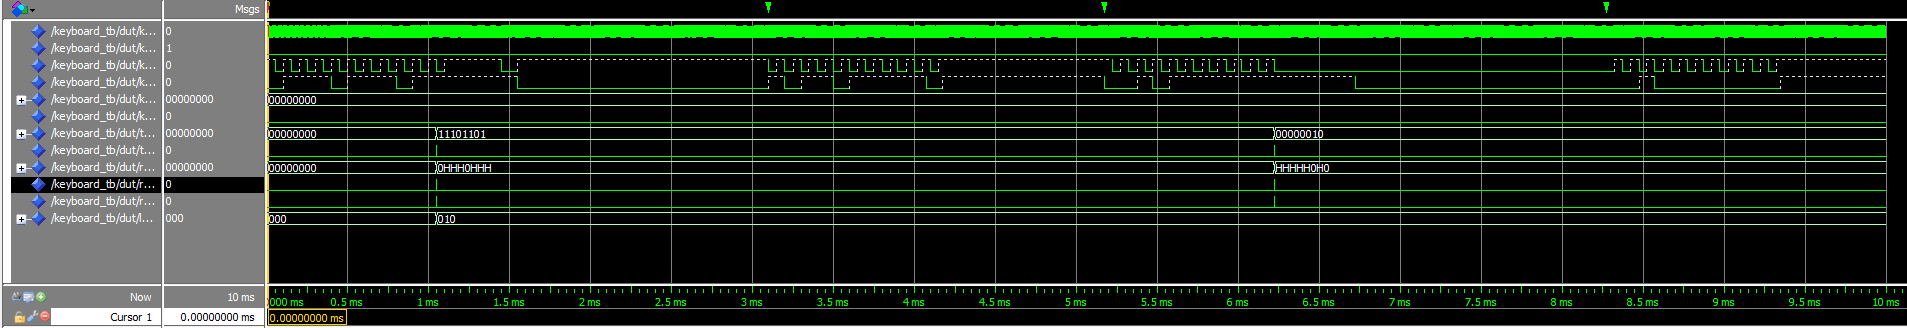
\includegraphics[width=1\textwidth]{assets/keyboard_tb}
			\captionof{figure}{Signalverlauf Keyboard Testbench}
		\end{center}
	
	
	\section{RamAccess\_tb}
		Zum Testen des RamAccess Moduls werden drei Bytes in den Speicher geschrieben. Danach werden sie sequenziell wieder ausgelesen und es wird geprüft, ob die Daten korrekt sind.
		\begin{center}
				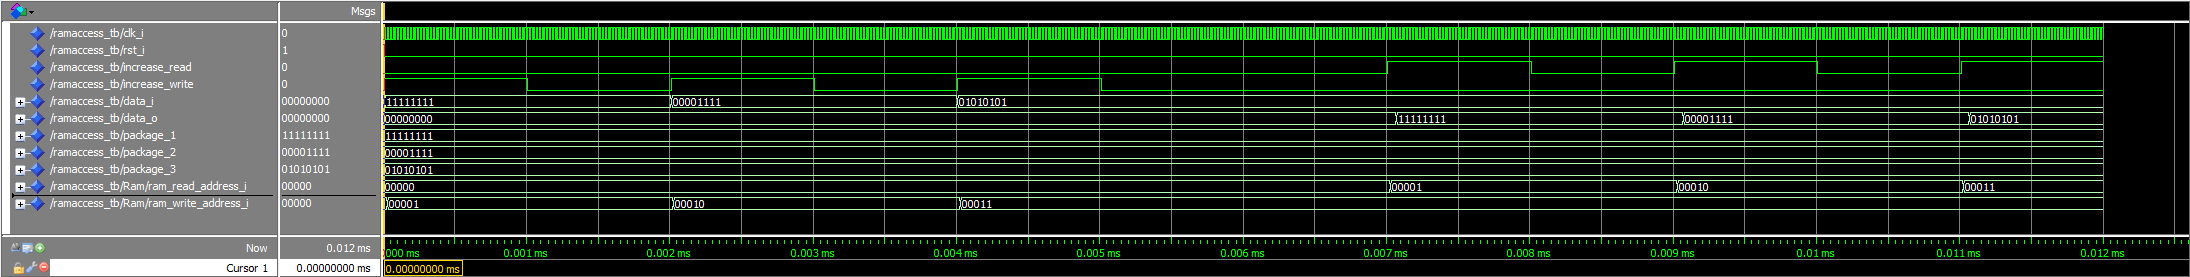
\includegraphics[width=1\textwidth]{assets/ramaccess_tb}
			\captionof{figure}{Signalverlauf RamAccess Testbench}
		\end{center}

	\section{CryptoNotepad\_tb}
		In der TLE Testbench wird das Zusammenspiel aller Module getestet. Zuerst muss hierfür 20ms auf die Initialisierung des Displays gewartet werden. Danach werden zwei Tastenanschläge simuliert. Jeweils mit korrektem Break Paket und anschließender Wiederholung des Make Codes. 
		Nach Empfangen des Tastendrucks werden die Daten wie erwartet in das Ram geschrieben und anschließend vom Display ausgelesen.
		\begin{center}
			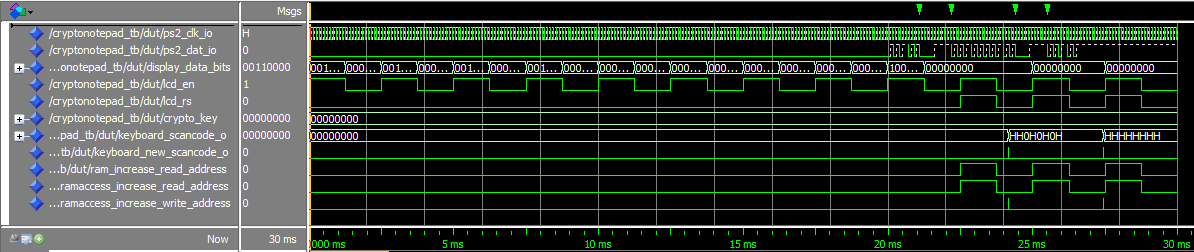
\includegraphics[width=1\textwidth]{assets/CryptoNotepad_tb}
			\captionof{figure}{Signalverlauf TLE Testbench}
		\end{center}
		
\chapter{Fazit}
	Leider sind die verwendeten Werkzeuge nicht zeitgemäß. Sowohl Quartus II als auch Modelsim werden in veralteten Versionen benutzt, welche den Arbeitsfluss extrem verlangsamen.
	Ohne VHDL Erfahrung war es zu Anfang recht schwer zu entscheiden, auf welcher Ebene modularisiert werden soll. Nach bestandener Klausur fiel es leichter.

\end{document}
